Środowisko symulacyjne zostało napisane w języku Python i bibliotekach pygame\cite{dokPygame} i pygame\_gui\cite{dokPygameGui},
zapewniające obsługę graficznego interfejsu użytkownika. 
\begin{lstlisting}[language=Python,caption=Uruchomienie aplikacji,label={kodPythonStartApki}]
if __name__ == '__main__':
    app = App()
    app.main()
\end{lstlisting}

\textbf{Obsługa mapy}

Dla logicznego podzielenia programu została napisana główna klasa programu o nazwie App.
Takie podejście pozwoliło na odseparowanie poszczególnych stanów w aplikacji. W pierwszej kolejności konstruktor obiektu aplikacji, generuje okno, tworzy 
graficzne elementy użytkownika oraz ustawia odpowiednie flagi informujące o stanie aplikacji. 
Dalej wywoływana jest funkcja main wczytująca odpowiednią mapę z pliku a następnie uruchamiająca główną pętle programu działającą w 60 klatkach na sekundę.

\begin{figure}[H]
	\centering
	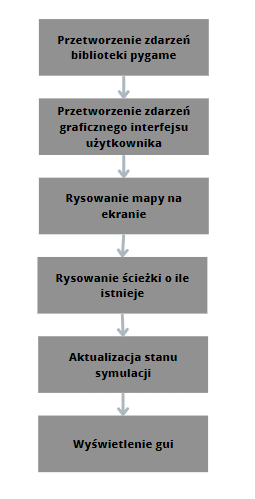
\includegraphics[width=6cm]{pages/implementacja/zdjecia/schematPetliApki.png}
	\caption{Schemat głównej pętli programu}
	\label{fig:schematPetliGlownej}
\end{figure}

Aby uprościć sobie symulowanie różnych scenariuszy i rozmiarów map otoczenia, ta ładowana jest ze wskazanego w 
programie pliku. Wskazany plik jest w formacie josn i podzielony jest na dwie sekcje. 
Pierwsza dostarcza informacje o samej mapie, natomiast druga o poruszającym się po niej robocie. Sekcja mapy zawiera lokalizacje do pliku tekstowego z zapisanymi elementami. 

\begin{lstlisting}[language=Python,caption=Uruchomienie aplikacji,label={kodPythonWczytanieMapy}]
(self.map, self.robot) = MapLoader.fromJson("maps/m02.json")
\end{lstlisting}
Ładowaniem wszystkich tych informacji zajmuje się specjalna metoda w klasie wywołana przed uruchomieniem pętli głównej. 
Wczytywana mapa jest w postaci siatki i stałym rozmiarze każdego elementu. Symulator rozróżnia kilka typów węzłów:
\begin{itemize}
	\item brak elementu - możliwy przejazd 
	\item ściana - przeszkoda do ominięcia przez algorytm
	\item punkt początkowy - punkt, od którego rozpoczyna się wyznaczanie ścieżki, zdefiniowany przez użytkownika
	\item punkt końcowy - analogicznie jak w poprzednim przypadku
	\item ścieżka - element wyznaczonej ścieżki
\end{itemize}

Wszystkie wymienione typy zapisane są w klasie Tile, reprezentującej pojedynczy rysowany i zapisywany do pliku kwadrat.
Użytkownik może w każdej chwili działania aplikacji edytować mapę. Przed zamknięciem aplikacji 
zaktualizowana mapa zapisywana jest do pliku. Wyjątkiem jest obiekt będący elementem ścieżki. 
Ten nie jest zapisywany do pliku, ponieważ generowany jest dynamicznie i służy tylko do reprezentacji wygenerowanej ścieżki.

\textbf{Wyznaczanie ścieżki i symulacja}


Po załadowaniu program oczekuje na akcje użytkownika i ewentualne uruchomienie wyznaczania ścieżki lub całej symulacji.
\begin{lstlisting}[language=Python,caption=Uruchomienie aplikacji,label={kodPythonWyznaczenieSciezki}]
elif ev.ui_element == self._startAStar:
    star = AStar(self.map.map, self.map.getSize())
    star.diagonalJump(self._diagonalJump)
    star.diagolnalCorrection(self._diagonalCorrextion)
    self.path       = star.findPath2(Node(self.map.getStartCords()), Node((self.map.getEndCords())))
    self._pathExist = True
    self.robot.stopSimulation()
    self.robot.hideRobot()
\end{lstlisting}

Po kliknięciu w przycisk odpowiadający za wyznaczenie i pokazanie ścieżki, program tworzy obiekt 
wyznaczający trasę i ustawia dodatkowe opcje algorytmu (np. skok po przekątnych). 
Dalej pobierana jest wyznaczona trasa będąca tablicą kolejnych punktów, po których należy przejść aby dojść do celu.
Na końcu ustawiana jest odpowiednia flaga programu, zatrzymywana jest symulacja i ukrywany jest robot (mamy nowo wyznaczoną trasę).
Przycisk uruchamiający symulacje sprawdza czy istnieje ścieżka i w razie potrzeby ją generuje. Następnie trasa podawana 
jest do obiektu robota odpowiadającego za symulacje i dalej symulacja jest uruchamiana.

\textbf{Przejście robota po ścieżce}

Symulator robota pobiera pierwszy punkt, do którego ma dotrzeć. Zmiana pozycji odbywa się poprzez regulator typu P z 
ustawioną nastawą na wskazany punkt. Wartość wzmocnienia proporcjonalnego wczytana jest z pliku mapy i oznaczona jest jako szybkość robota.
Dalszy etap to sprawdzenie czy symulowany robot dotarł do celu. 
\begin{lstlisting}[language=Python,caption=Uruchomienie aplikacji,label={kodPythonSprawdzenieCeluRobota}]
if abs(deltaPos0) < 0.2 and abs(deltaPos1) < 0.2:
            self._currentTarget -= 1
\end{lstlisting}
Realizowane jest to poprzez sprawdzenie czy wartość bezwzględna z różnicy aktualnej oraz docelowej pozycji jest mniejsza niż 0,1.
Po osiągnięciu punkt ustawiany jest nowy indeks wskazujący na kolejny cel.
Jeżeli na początku aktualizacji indeks jest ujemny to robot przejechał po całej wyznaczonej trasie.

\textbf{Komunikacja z robotem}
% polaczenie z robotem po tcp

Po wyznaczeniu ścieżki symulator na polecenie użytkownika może połączyć się ze zbudowanym robotem aby ten osiągnął założony cel.
Zgodnie ze schematem \cite{sch:ogolnyRozwiazania} robot po połączeniu z siecią WiFi i utworzeniu serwera TCP oczekuje na wysyłane komendy.
Aplikacja podczas uruchamiania się tworzy gniazdo, które potem zostanie wykorzystane do połączenia. 
\begin{lstlisting}[language=Python,caption=Utworzone gniazdo,label={kodPythonGniazdo}]
self._robotSocket       = socket.socket(socket.AF_INET, socket.SOCK_STREAM)
\end{lstlisting}
Dla zwiększenia elastyczności utworzone są dwa pola tekstowe pozwalające na wprowadzenie adresu ip oraz portu z uruchomionym serwerem.
Po wprowadzeniu wymaganych danych operator może spróbować nawiązać połączenie z robotem poprzez specjalny przycisk.


\begin{lstlisting}[language=Python,caption=Nawiązanie połączenia,label={kodPythonGniazdo}]
if self._robotSocketFlag is True:
self._robotSocket.close()

print(f"Laczenie z robotem {(self._textRobotIp.get_text(), int(self._textRobotPort.get_text()))}")
self._robotSocket.settimeout(1)
try:
    self._robotSocket.connect((self._textRobotIp.get_text(), int(self._textRobotPort.get_text())))
    self._robotSocketFlag = True
    self._sendCommandToRobot("setMode auto")
    print("Podlaczono!!!")
except Exception as err:
    self._robotSocketFlag = False
    print(f"Blad polaczenia z robotem")
    print(err)
\end{lstlisting}
W pierwszej kolejności sprawdzana jest flaga informująca o stanie połączenia, jeżeli jest aktywne to połączenie jest zamykane.
Na utworzonym gnieździe wywoływana jest funkcja connect z wprowadzonymi przez użytkownika parametrami.
Cała operacja zamknięta jest w bloku try..except a więc jeżeli program nie połączy się z robotem to wyświetlana jest odpowiednia informacja. 
Podczas łączenia należy zwracać uwagę na podsieci, w których jest robot i sterujący laptop. 
Dodatkowo robot posiada dynamiczne ip co zostało szerzej opisane w rozdziale o oprogramowaniu robota.
Jeżeli żaden wyjątek nie został rzucony to wysyłana jest pierwsza komenda ustawiająca tryb robota na automatyczny.


\begin{lstlisting}[language=Python,caption=Wysyłanie komendy do robota,label={kodPythonSendCmd}]
def _sendCommandToRobot(self, cmd):
    if self._robotSocketFlag is False:
        print("Robot nie podlaczony!!")
        return
    
    try:
        self._robotSocket.send(str.encode(cmd))
    except OSError as err:
        print("Robot nie podlaczony!!!")
        self._robotSocket.close()
        self._robotSocketFlag = False
        return
\end{lstlisting}
Program może wysłać dowolną komendę robota poprzez metodę sendCommandToRobot. 
Podobnie jak przy połączeniu, metoda wysyłająca dane może rzucić wyjątek o braku połączenia. W takim przypadku
wyświetlana jest odpowiednia informacja i resetowana jest flaga połączenia. 


% TODO: tu kiedys o wysyłanych komendach ze sciezka

% TODO: zdjecie z calego program, efekt
\textbf{Finalna wersja programu}

Na poniższym zrzucie widać uruchomiony program z trwającą symulacją. Po prawej stronie został umieszczony panel 
z interfejsem użytkownika. Po lewej stronie widoczna jest wczytana mapa. 
Kolorem niebieskim został oznaczony punkt startowy a czerwonym końcowy.
Żółte kratki oznaczają wyznaczoną przez algorytm ścieżkę, po której przejdzie robot. Szare pola to przeszkody, które robot ma ominąć. 
Robot oznaczony jest przez jasno-zielone koło, które przesuwa się po polu. 

\begin{figure}[H]
	\centering
	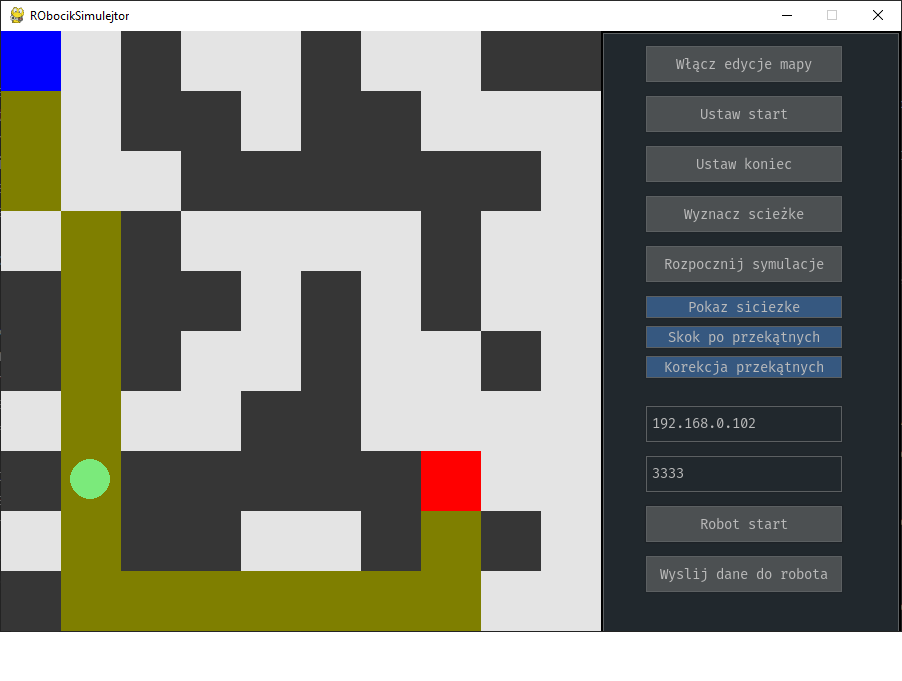
\includegraphics[width=16cm]{pages/implementacja/zdjecia/calyProgram.png}
	\caption{Widok finalnej wersji programu}
	\label{fig:finalnaWersjaProgramu}
\end{figure}